
\pagebreak



% 
% 
\section{Stack design } \label{sec:U5_d_stack_design}

% Plots of the isomer-to-ground state ratios measured in this work are presented here, in comparison with literature data and reaction modeling codes 
% \cite{Michel1978,Kopecky1993,Zarie2006a,Khandaker2009}.





% Combined table
% Please add the following required packages to your document preamble:
% \usepackage{booktabs}
\begin{table*}[h!]
\centering
\caption{Specifications of the 25\,MeV and 55\,MeV target stack designs in the present work. The proton beam enters the stack upstream of the SS-5 and SS-3 profile monitors, respectively, and travels through the stack in the order presented here. The 6061 aluminum degraders have a measured density of approximately 2.68 $\pm$ 0.03 g/cm$^3$. Their areal densities were determined using the variance minimization techniques described  in this work  and an earlier paper\,\cite{Voyles2018a}. 
% the earlier paper by Graves \etal\\,\cite{Graves2016}.
A 316 stainless steel foil is inserted at both the front and rear of each target stack as a monitor of the beam's spatial profile, by developing radiochromic film (Gafchromic EBT3) after end-of-bombardment (EoB).}
\label{tab:fe_stack_table}
\small
\resizebox{\textwidth}{!}{%
\begin{tabular}{@{}llll|llll@{}}
\toprule\toprule
% Target Layer       & Nominal Thickness & Measured thickness (mg/cm\textasciicircum 2) & Thickness Uncertainty (\%) \\ \midrule
25\,MeV Target layer            & \begin{tabular}[c]{@{}l@{}}Measured \\ thickness\end{tabular} & \begin{tabular}[c]{@{}l@{}}Measured\\areal density\\(mg/cm$^2$)\end{tabular} & \begin{tabular}[c]{@{}l@{}}Uncertainty \\ in areal\\ density  (\%)\end{tabular} & 55\,MeV Target layer            & \begin{tabular}[c]{@{}l@{}}Measured \\ thickness\end{tabular} & \begin{tabular}[c]{@{}l@{}}Measured\\areal density\\(mg/cm$^2$)\end{tabular} & \begin{tabular}[c]{@{}l@{}}Uncertainty \\ in areal\\ density  (\%)\end{tabular} \\
\midrule
SS profile monitor SS-5 & 130.94 \mmicro m                                              & 100.57                                                                      & 0.17                                                                      & SS profile monitor SS-3 & 130.9 \mmicro m                                               & 100.48                                                                      & 0.17                                                                      \\
Fe-08                   & 26.25 \mmicro m                                               & 19.69                                                                       & 0.17                                                                      & Fe-01                   & 25.75 \mmicro m                                               & 20.22                                                                       & 0.21                                                                      \\
Ti-14                   & 25.01 \mmicro m                                               & 10.87                                                                       & 0.36                                                                      & Ti-01                   & 25.88 \mmicro m                                               & 11.09                                                                       & 0.16                                                                      \\
Cu-14                   & 24.01 \mmicro m                                               & 17.49                                                                       & 0.40                                                                      & Cu-01                   & 28.81 \mmicro m                                               & 22.40                                                                       & 0.11                                                                      \\
Al Degrader E-09        & 256.5 \mmicro m                                               & --                                                                          & --                                                                        & Al Degrader A-1         & 2.24 mm                                                       & --                                                                          & --                                                                        \\
Fe-09                   & 26.5 \mmicro m                                                & 19.90                                                                       & 0.09                                                                      & Fe-02                   & 25.5 \mmicro m                                                & 19.91                                                                       & 0.13                                                                      \\
Ti-15                   & 23.81 \mmicro m                                               & 10.97                                                                       & 0.11                                                                      & Ti-02                   & 25.74 \mmicro m                                               & 10.94                                                                       & 0.24                                                                      \\
Cu-15                   & 21.81 \mmicro m                                               & 17.63                                                                       & 0.46                                                                      & Cu-02                   & 28.75 \mmicro m                                               & 22.32                                                                       & 0.40                                                                      \\
Al Degrader H-01        & 127.09 \mmicro m                                              & --                                                                          & --                                                                        & Al Degrader A-2         & 2.24 mm                                                       & --                                                                          & --                                                                        \\
Fe-10                   & 26.5 \mmicro m                                                & 19.84                                                                       & 0.11                                                                      & Fe-03                   & 25.25 \mmicro m                                               & 20.00                                                                       & 0.27                                                                      \\
Ti-16                   & 24.6 \mmicro m                                                & 10.96                                                                       & 0.32                                                                      & Ti-03                   & 25.91 \mmicro m                                               & 11.25                                                                       & 0.15                                                                      \\
Cu-16                   & 22.01 \mmicro m                                               & 17.22                                                                       & 0.25                                                                      & Cu-03                   & 28.86 \mmicro m                                               & 22.49                                                                       & 0.20                                                                      \\
Fe-11                   & 27.26 \mmicro m                                               & 19.96                                                                       & 0.17                                                                      & Al Degrader C-1         & 0.97 mm                                                       & --                                                                          & --                                                                        \\
Ti-17                   & 25.01 \mmicro m                                               & 10.88                                                                       & 0.25                                                                      & Fe-04                   & 25.25 \mmicro m                                               & 19.93                                                                       & 0.33                                                                      \\
Cu-17                   & 29 \mmicro m                                                  & 21.91                                                                       & 0.33                                                                      & Ti-04                   & 25.84 \mmicro m                                               & 10.91                                                                       & 0.18                                                                      \\
Fe-12                   & 27.01 \mmicro m                                               & 20.03                                                                       & 0.12                                                                      & Cu-04                   & 28.78 \mmicro m                                               & 22.38                                                                       & 0.29                                                                      \\
Ti-18                   & 25.01 \mmicro m                                               & 11.00                                                                       & 0.87                                                                      & Al Degrader C-2         & 0.97 mm                                                       & --                                                                          & --                                                                        \\
Cu-18                   & 28.75 \mmicro m                                               & 22.33                                                                       & 0.14                                                                      & Fe-05                   & 25.64 \mmicro m                                               & 20.02                                                                       & 0.24                                                                      \\
Fe-13                  & 26.25 \mmicro m                                               & 20.05                                                                       & 0.16                                                                      & Ti-05                   & 25.86 \mmicro m                                               & 10.99                                                                       & 0.30                                                                      \\
Ti-19                   & 26.6 \mmicro m                                                & 11.01                                                                       & 0.22                                                                      & Cu-05                   & 28.77 \mmicro m                                               & 22.35                                                                       & 0.12                                                                      \\
Cu-19                   & 28.75 \mmicro m                                               & 22.32                                                                       & 0.19                                                                      & Al Degrader C-3         & 0.97 mm                                                       & --                                                                          & --                                                                        \\
Fe-14                   & 25.75 \mmicro m                                               & 20.11                                                                       & 0.19                                                                      & Fe-06                   & 25.75 \mmicro m                                               & 20.21                                                                       & 0.26                                                                      \\
Ti-20                   & 27.01 \mmicro m                                               & 11.06                                                                       & 0.35                                                                      & Ti-06                   & 25.5 \mmicro m                                                & 11.15                                                                       & 0.23                                                                      \\
Cu-20                   & 28.26 \mmicro m                                               & 22.34                                                                       & 0.28                                                                      & Cu-06                   & 28.83 \mmicro m                                               & 22.43                                                                       & 0.10                                                                      \\
SS profile monitor SS-6 & 131.5 \mmicro m                                               & 100.99                                                                      & 0.17                                                                      & Al Degrader C-4         & 0.97 mm                                                       & --                                                                          & --                                                                        \\
                        &                                                               &                                                                             &                                                                           & Fe-07                   & 25.76 \mmicro m                                               & 19.93                                                                       & 0.19                                                                      \\
                        &                                                               &                                                                             &                                                                           & Ti-07                   & 25.75 \mmicro m                                               & 11.17                                                                       & 0.33                                                                      \\
                        &                                                               &                                                                             &                                                                           & Cu-07                   & 28.76 \mmicro m                                               & 22.34                                                                       & 0.24                                                                      \\
                        &                                                               &                                                                             &                                                                           & Al Degrader H-02        & 127.04 \mmicro m                                              & --\cmmnt{34.51}                                                                       & --\cmmnt{0.20}                                                                      \\
                        &                                                               &                                                                             &                                                                           & SS profile monitor SS-4 & 131.21 \mmicro m                                              & 101.25                                                                      & 0.16                                                                     \\
 \bottomrule\bottomrule
\end{tabular}
}
\end{table*}


% 
% 
\section{Measured excitation functions} \label{sec:U5_d_xs_figures}

Figures of the cross sections measured in this work are presented here, in comparison with literature data
% \cite{Al-Abyad2009,A2006,Aleksandrov1987,barchuk1987excitation,Barrandon1975,Belhout2007,Brodzinski1971,Brodzinski1971a,daum1997investigation,Ditroi2005,Fink1990,Garrido2016,Graves2016,Greenwood1984,Grutter1982,Jung1987,Khandaker2009,Kim2014,Kopecky1993,Lagunas-Solar1979a,levkovski1991cross,MICHEL1997153,MICHEL1979a,Michel1980,Michel1978,Michel1985,Mills1992,Neumann1999a,Schoen1979a,Shahid2015,Sudar1994,Takacs1994a,Voyles2018a,PhysRev.162.1055,YashimaH2003,Zarie2006a,zhao1993measurement}.

% \comment{Add in CoH model output from Toshihiko to all plots}


% 
% 
% 
% % Prevent ''overfull hbox'' warnings for < 5pt overflow 
% % \hfuzz=10pt 
% 
% \begin{figure*}
%     \sloppy
%     \centering
%     \subfloat{
%         \centering
% %         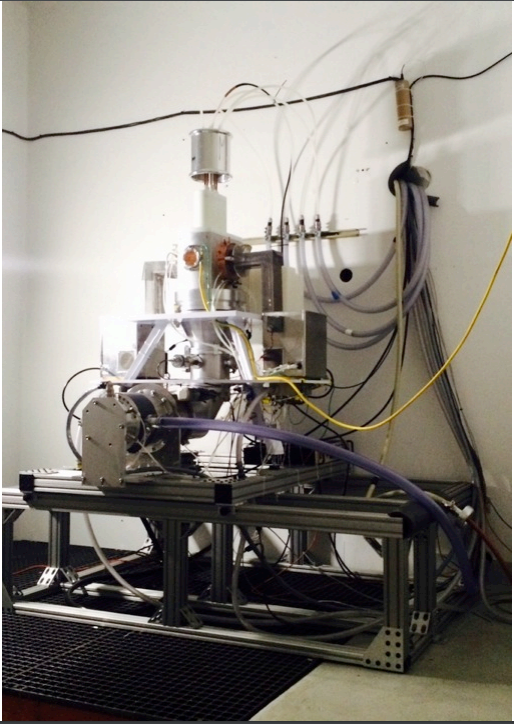
\includegraphics[width=\columnwidth]{./figures/Capture.PNG}
%         \subfigimg[width=0.496\textwidth]{}{./figures/48Cr.pdf}{50}
% %         \caption{ Decay curve for the isomeric transition of \ce{^{115m}In}.}
% %         \refstepcounter{subfigure}
% %          \label{fig:51Cr}%
% %         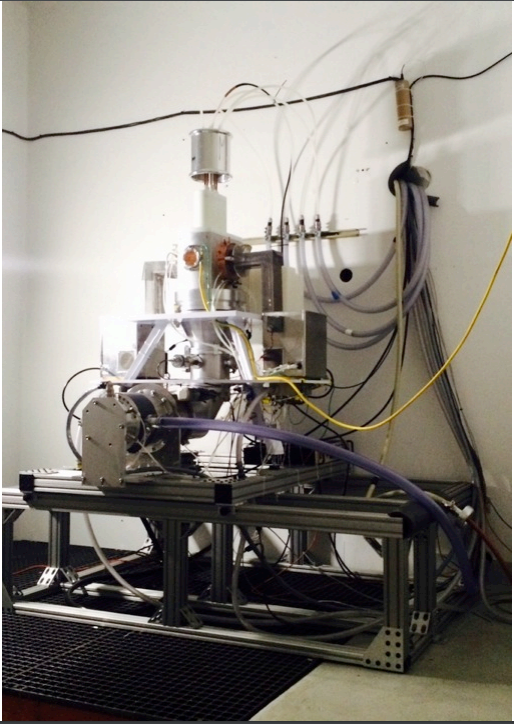
\includegraphics[width=\columnwidth]{./figures/Capture.PNG}
% %         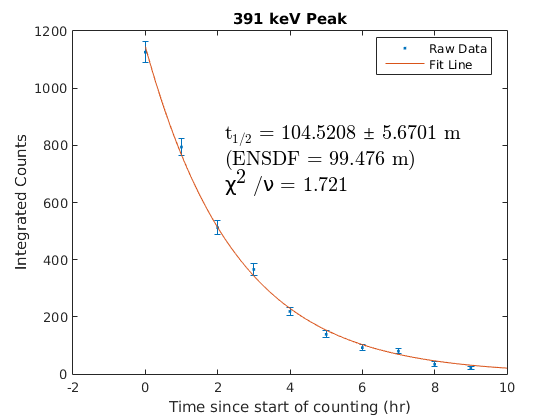
\includegraphics[scale=0.6]{./figures/391keV_curve2.png}
%         \subfigimg[width=0.496\textwidth]{}{./figures/48V_ind.pdf}{50}
% %         \caption{ Decay curve for the isomeric transition of \ce{^{113m}In}.}
% %         \refstepcounter{subfigure}
% %          \label{fig:52Mn}
%    \hspace{-10pt}}%
%     \\
%     \subfloat{
%         \centering
% %         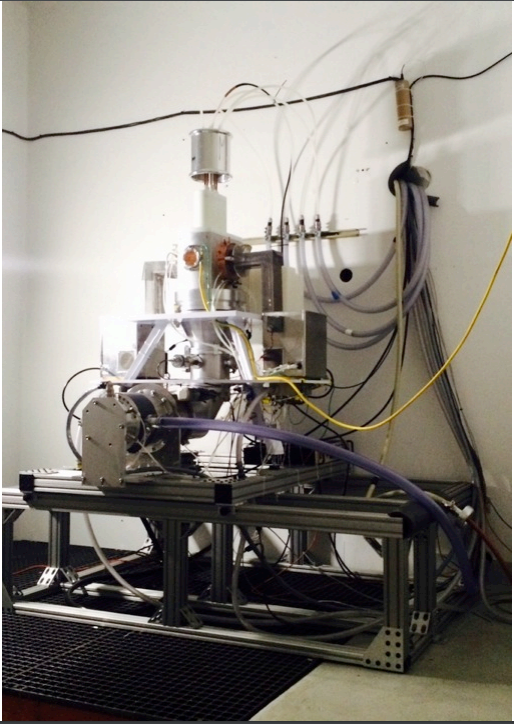
\includegraphics[width=\columnwidth]{./figures/Capture.PNG}
%         \subfigimg[width=0.496\textwidth]{}{./figures/48V_cum.pdf}{50}
% %         \caption{ Decay curve for the isomeric transition of \ce{^{115m}In}.}
% %         \refstepcounter{subfigure}
% %          \label{fig:52gMn}%
% %         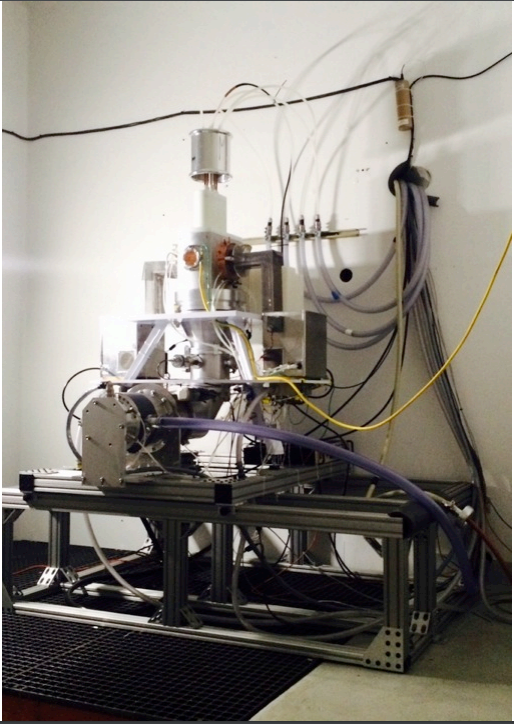
\includegraphics[width=\columnwidth]{./figures/Capture.PNG}
% %         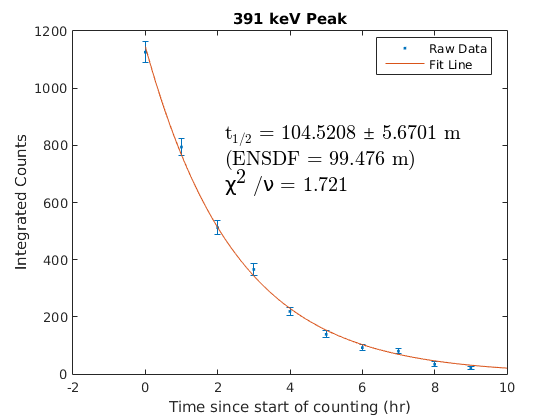
\includegraphics[scale=0.6]{./figures/391keV_curve2.png}
%         \subfigimg[width=0.496\textwidth]{}{./figures/49Cr.pdf}{50}
% %         \caption{ Decay curve for the isomeric transition of \ce{^{113m}In}.}
% %         \refstepcounter{subfigure}
% %          \label{fig:52mMn}
%    \hspace{-10pt}}%
%     \\
%     \subfloat{
%         \centering
% %         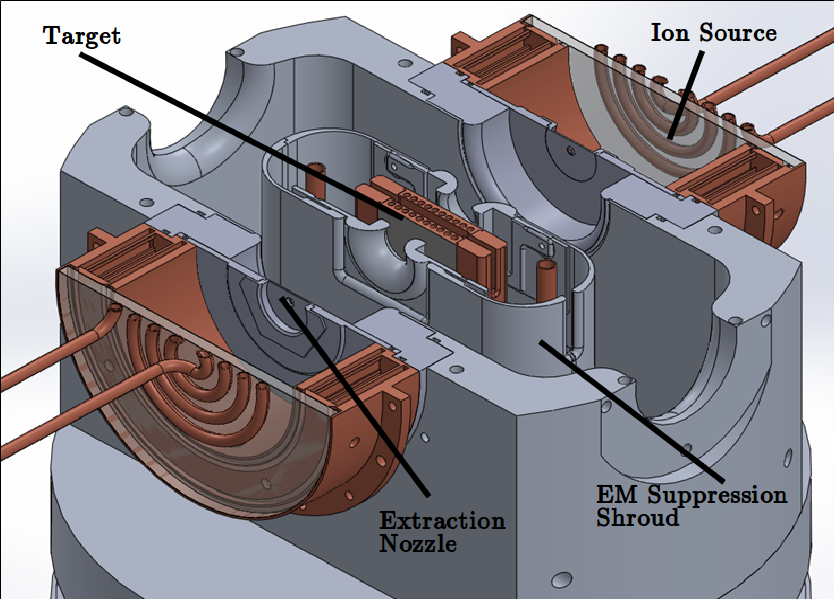
\includegraphics[width=\textwidth]{./figures/target2.png}
%         \subfigimg[width=0.496\textwidth]{}{./figures/51Cr_ind.pdf}{50}
% %         \caption{Decay curve for the $\beta^-$ decay of \ce{^{116}In}.}
%         %         \refstepcounter{subfigure}
% %          \label{fig:54Mn}
% %
% %         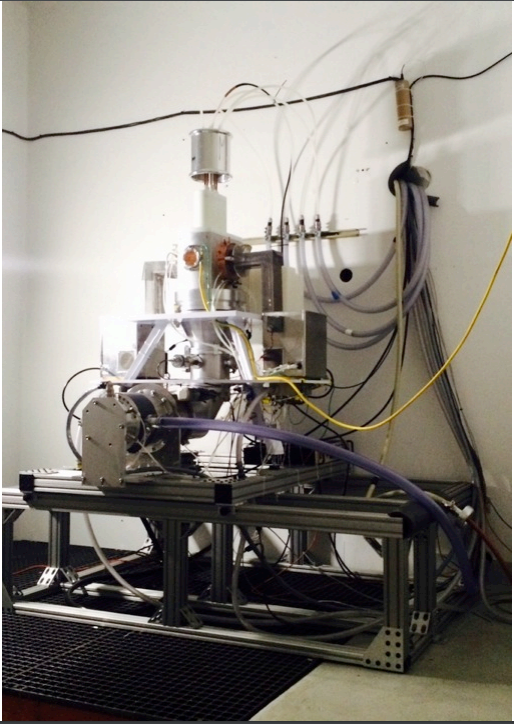
\includegraphics[width=\columnwidth]{./figures/Capture.PNG}
%         \subfigimg[width=0.496\textwidth]{}{./figures/51Cr_cum.pdf}{50}
% %         \caption{ Decay curve for the $\beta^+$ decay of \ce{^{64}Cu}.}
% %         \refstepcounter{subfigure} 
% %         \label{fig:55Co}
%    \hspace{-10pt}}%
% %     \caption{Decay curves used to verify photopeak transition assignment. (a) Decay curve for the isomeric transition of \ce{^{115m}In}, (b) decay curve for the isomeric transition of \ce{^{113m}In}, (c) decay curve for the $\beta^-$ decay of \ce{^{116}In}, and (d) decay curve for the $\beta^+$ decay of \ce{^{64}Cu}.}
%      \phantomcaption{}\label{fig:xs_curves_p1}
% \end{figure*}
% 
% 
% 
% 
% \begin{figure*}
%     \centering
%     \subfloat{
%         \centering
% %         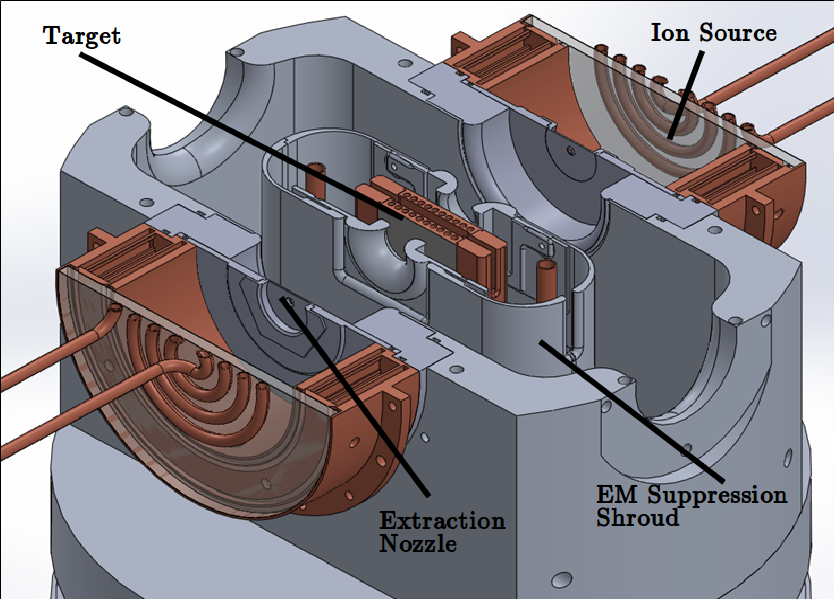
\includegraphics[width=\textwidth]{./figures/target2.png}
%         \subfigimg[width=0.496\textwidth]{}{./figures/52gMn.pdf}{50}
% %         \caption{Decay curve for the $\beta^-$ decay of \ce{^{116}In}.}
%         %         \refstepcounter{subfigure}
% %          \label{fig:56Ni}
% %
% %         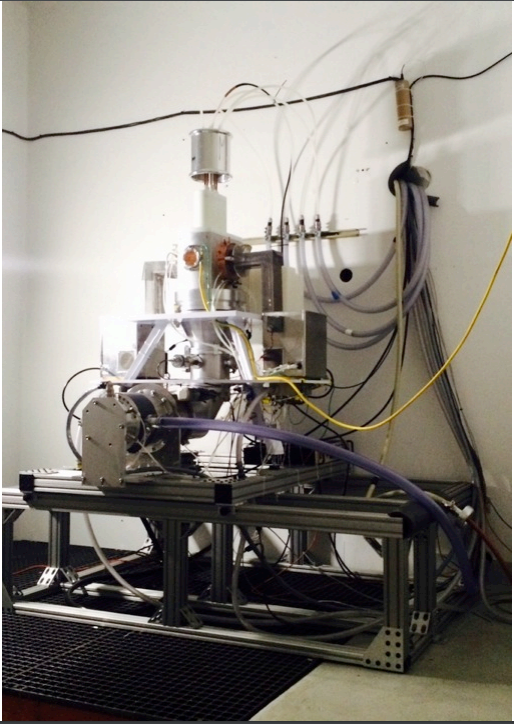
\includegraphics[width=\columnwidth]{./figures/Capture.PNG}
%         \subfigimg[width=0.496\textwidth]{}{./figures/52Fe.pdf}{50}
% %         \caption{ Decay curve for the $\beta^+$ decay of \ce{^{64}Cu}.}
% %         \refstepcounter{subfigure}
% %         \label{fig:57Co}
%    \hspace{-10pt}}%
%     \\
%     \subfloat{
%         \centering
% %         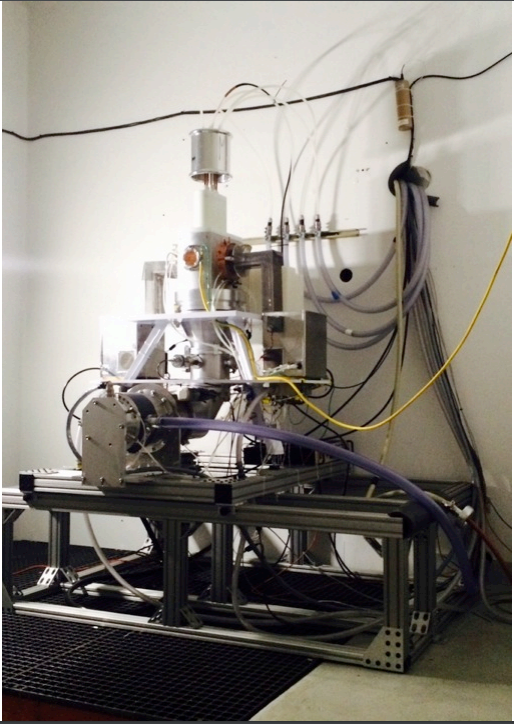
\includegraphics[width=\columnwidth]{./figures/Capture.PNG}
%         \subfigimg[width=0.496\textwidth]{}{./figures/54Mn.pdf}{50}
% %         \caption{ Decay curve for the isomeric transition of \ce{^{115m}In}.}
% %         \refstepcounter{subfigure}
% %          \label{fig:57Ni}%
% %         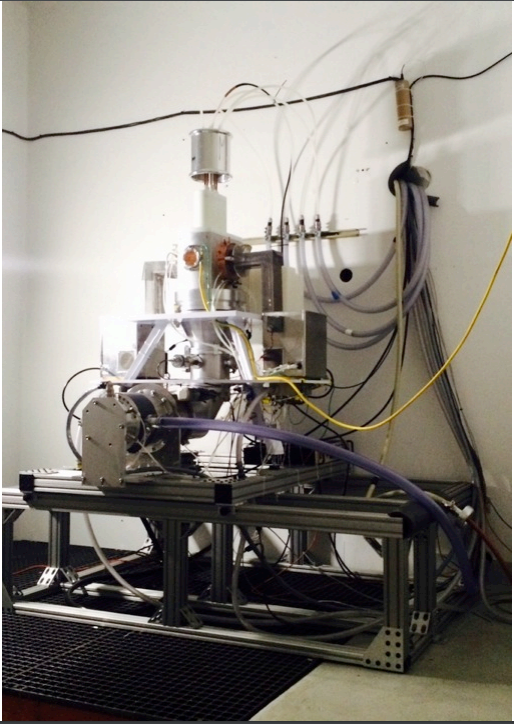
\includegraphics[width=\columnwidth]{./figures/Capture.PNG}
% %         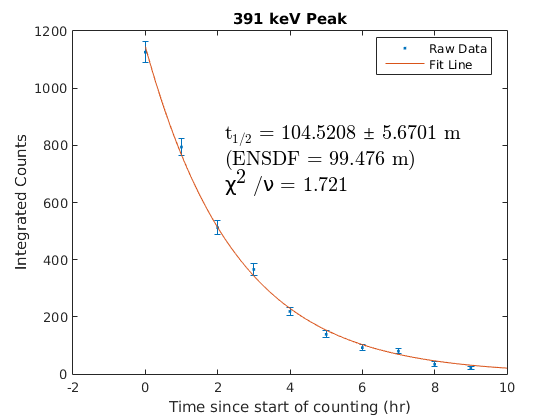
\includegraphics[scale=0.6]{./figures/391keV_curve2.png}
%         \subfigimg[width=0.496\textwidth]{}{./figures/55Co.pdf}{50}
% %         \caption{ Decay curve for the isomeric transition of \ce{^{113m}In}.}
% %         \refstepcounter{subfigure}
% %          \label{fig:58Co}
%    \hspace{-10pt}}%
%     \\
%     \subfloat{
%         \centering
% %         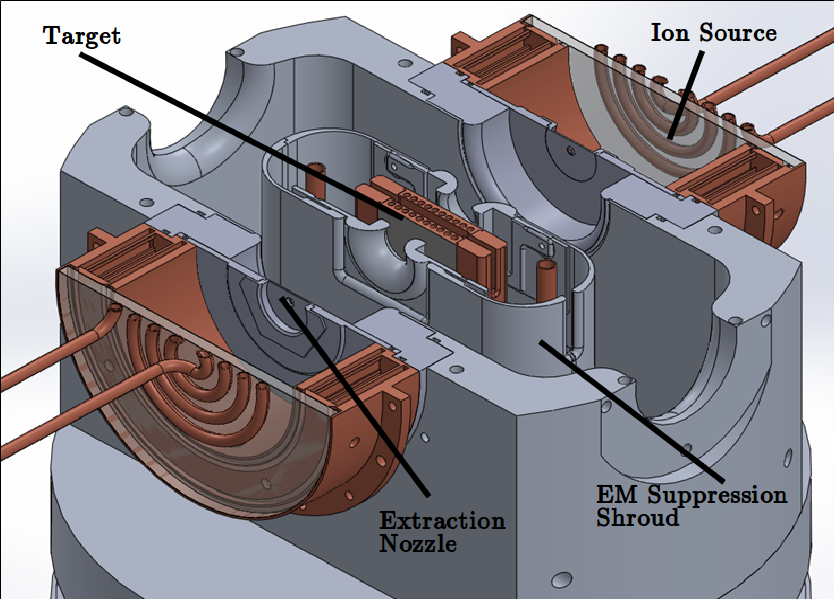
\includegraphics[width=\textwidth]{./figures/target2.png}
%         \subfigimg[width=0.496\textwidth]{}{./figures/56Mn.pdf}{50}
% %         \caption{Decay curve for the $\beta^-$ decay of \ce{^{116}In}.}
%         %         \refstepcounter{subfigure}
% %          \label{fig:58gCo}
% %
% %         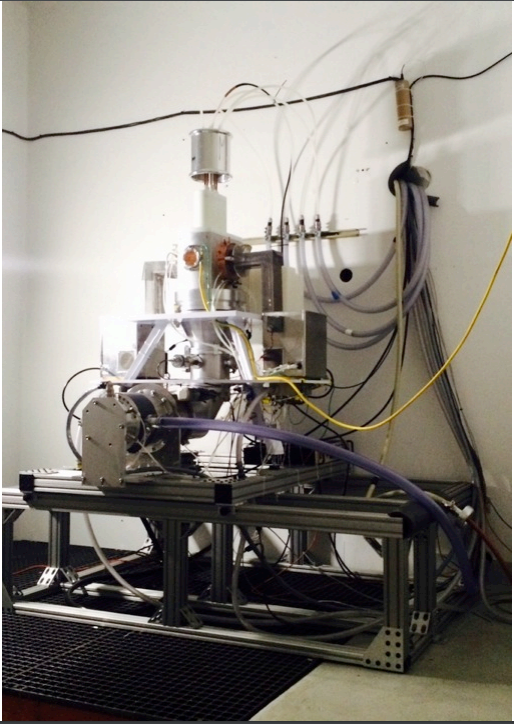
\includegraphics[width=\columnwidth]{./figures/Capture.PNG}
%         \subfigimg[width=0.496\textwidth]{}{./figures/56Co.pdf}{50}
% %         \caption{ Decay curve for the $\beta^+$ decay of \ce{^{64}Cu}.}
% %         \refstepcounter{subfigure}
% %         \label{fig:58mCo}
%    \hspace{-10pt}}%
% %     \caption{Decay curves used to verify photopeak transition assignment. (a) Decay curve for the isomeric transition of \ce{^{115m}In}, (b) decay curve for the isomeric transition of \ce{^{113m}In}, (c) decay curve for the $\beta^-$ decay of \ce{^{116}In}, and (d) decay curve for the $\beta^+$ decay of \ce{^{64}Cu}.}
%      \phantomcaption{}\label{fig:xs_curves_p2}
% \end{figure*}
% 
% 
% 
% \begin{figure*}
%     \centering
%     \subfloat{
%         \centering
% %         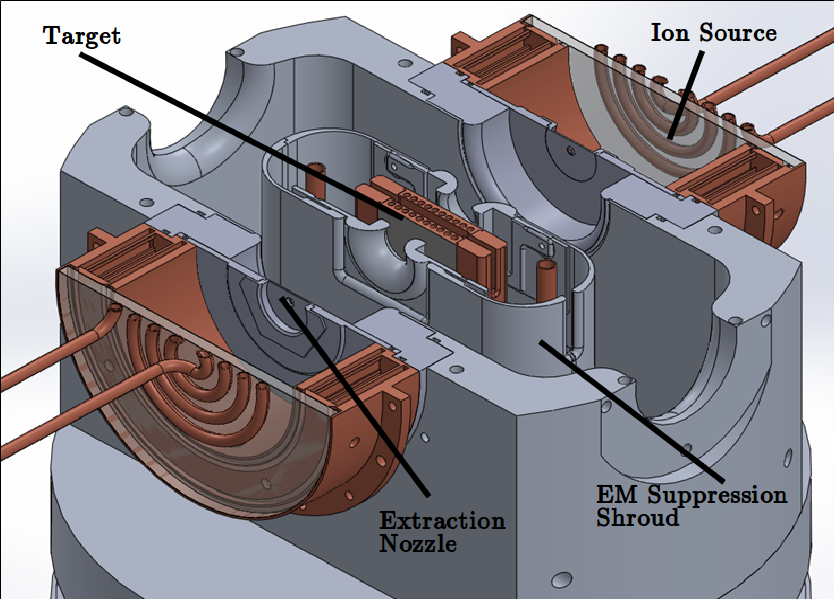
\includegraphics[width=\textwidth]{./figures/target2.png}
%         \subfigimg[width=0.496\textwidth]{}{./figures/57Co.pdf}{50}
% %         \caption{Decay curve for the $\beta^-$ decay of \ce{^{116}In}.}
%         %         \refstepcounter{subfigure}
% %          \label{fig:59Fe}
% %
% %         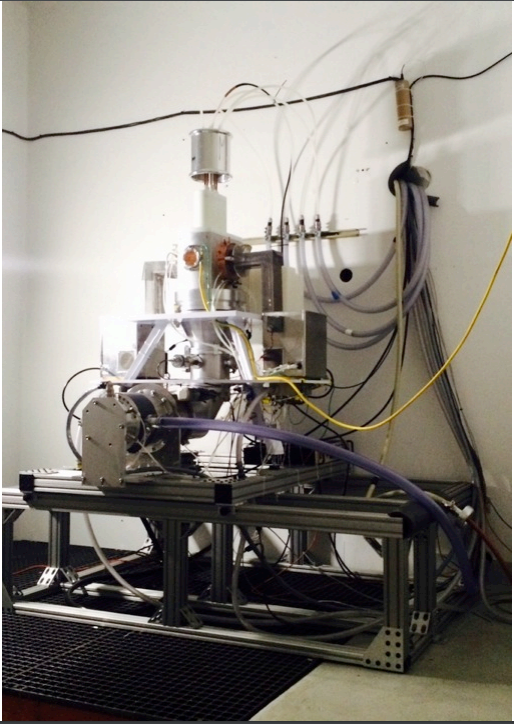
\includegraphics[width=\columnwidth]{./figures/Capture.PNG}
%         \subfigimg[width=0.496\textwidth]{}{./figures/58mCo.pdf}{50}
% %         \caption{ Decay curve for the $\beta^+$ decay of \ce{^{64}Cu}.}
% %         \refstepcounter{subfigure} 
% %         \label{fig:60Co}
%    \hspace{-10pt}}%
%     \\
%     \subfloat{
%         \centering
% %         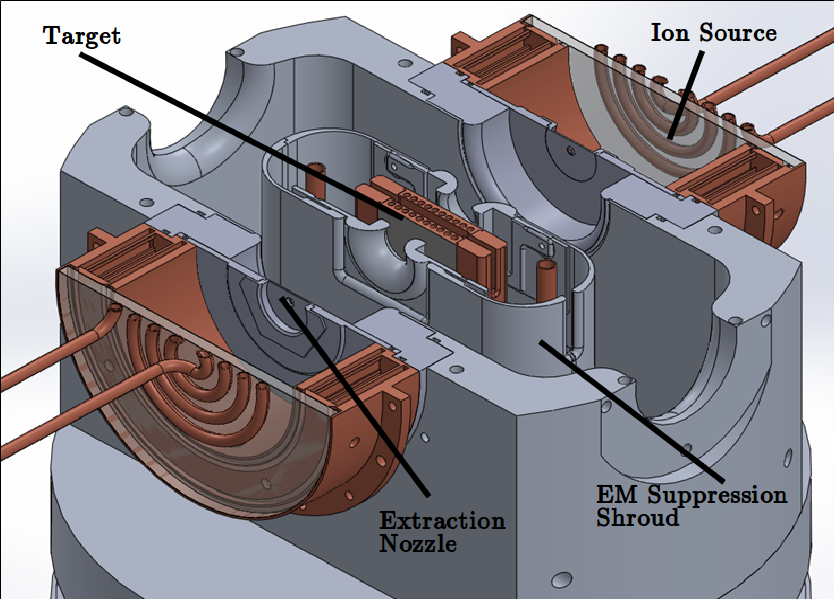
\includegraphics[width=\textwidth]{./figures/target2.png}
%         \subfigimg[width=0.496\textwidth]{}{./figures/58gCo.pdf}{50}
% %         \caption{Decay curve for the $\beta^-$ decay of \ce{^{116}In}.}
%         %         \refstepcounter{subfigure}
% %          \label{fig:61Cu}
% %
% %         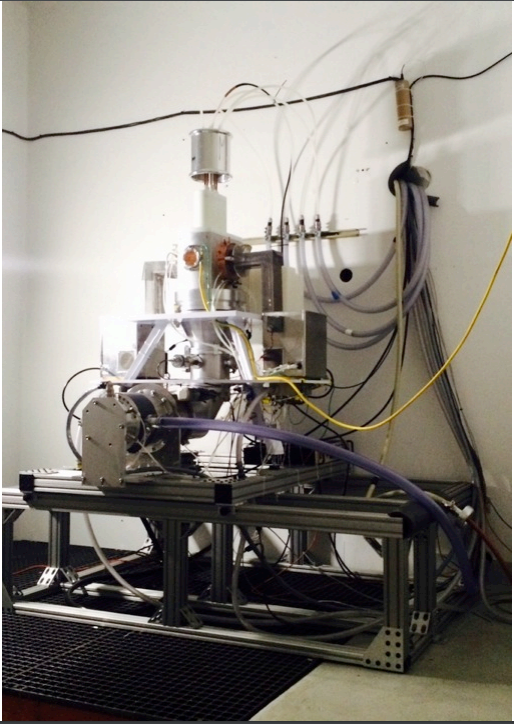
\includegraphics[width=\columnwidth]{./figures/Capture.PNG}
%         \subfigimg[width=0.496\textwidth]{}{./figures/58Co.pdf}{50}
% %         \caption{ Decay curve for the $\beta^+$ decay of \ce{^{64}Cu}.}
% %         \refstepcounter{subfigure}
% %         \label{fig:64Cu}
%    \hspace{-10pt}}%
%     \\
%     \subfloat{
%         \centering
% %         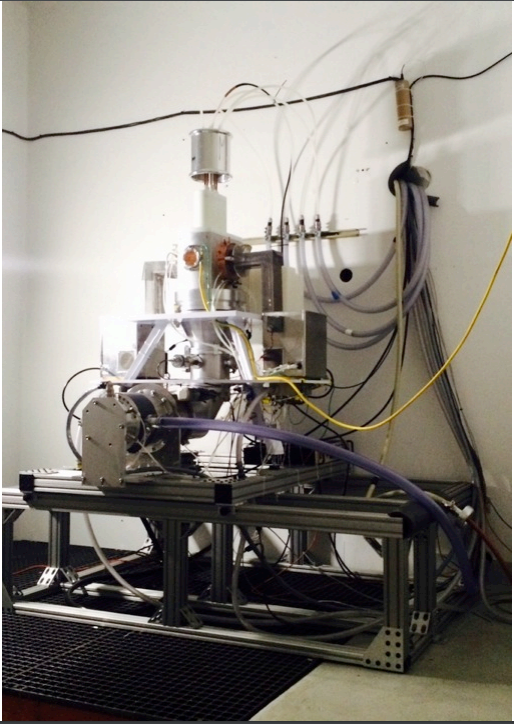
\includegraphics[width=\columnwidth]{./figures/Capture.PNG}
%         \subfigimg[width=0.496\textwidth]{}{./figures/54MnCu.pdf}{50}
% %         \caption{ Decay curve for the isomeric transition of \ce{^{115m}In}.}
% %         \refstepcounter{subfigure}
% %          \label{fig:82mRb}%
% %         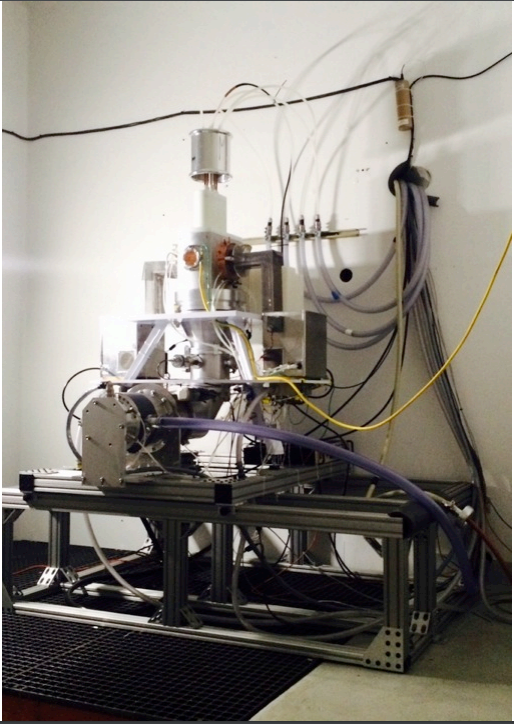
\includegraphics[width=\columnwidth]{./figures/Capture.PNG}
% %         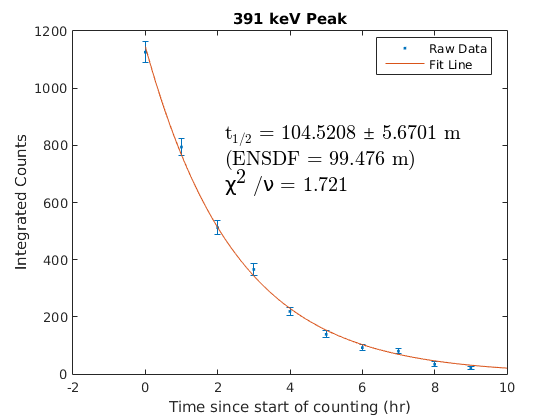
\includegraphics[scale=0.6]{./figures/391keV_curve2.png}
%         \subfigimg[width=0.496\textwidth]{}{./figures/57Ni.pdf}{50}
% %         \caption{ Decay curve for the isomeric transition of \ce{^{113m}In}.}
% %         \refstepcounter{subfigure}
% %          \label{fig:83Sr}
%    \hspace{-10pt}}%
% %     \caption{Decay curves used to verify photopeak transition assignment. (a) Decay curve for the isomeric transition of \ce{^{115m}In}, (b) decay curve for the isomeric transition of \ce{^{113m}In}, (c) decay curve for the $\beta^-$ decay of \ce{^{116}In}, and (d) decay curve for the $\beta^+$ decay of \ce{^{64}Cu}.}
%      \phantomcaption{}\label{fig:xs_curves_p3}
% \end{figure*}
% 
% 
% 
% \begin{figure*}
%     \centering
%     \subfloat{
%         \centering
% %         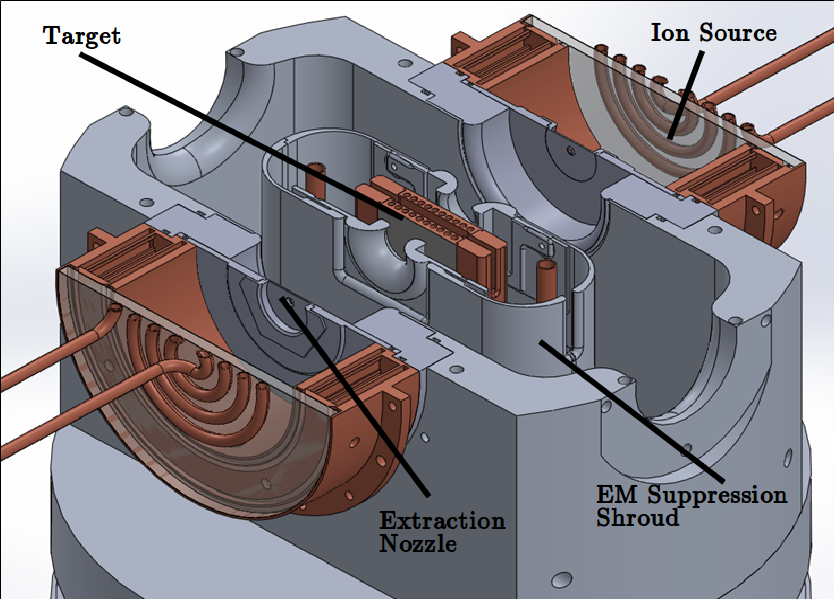
\includegraphics[width=\textwidth]{./figures/target2.png}
%         \subfigimg[width=0.496\textwidth]{}{./figures/57Co_ind.pdf}{50}
% %         \caption{Decay curve for the $\beta^-$ decay of \ce{^{116}In}.}
%         %         \refstepcounter{subfigure}
% %          \label{fig:85Y}
% %
% %         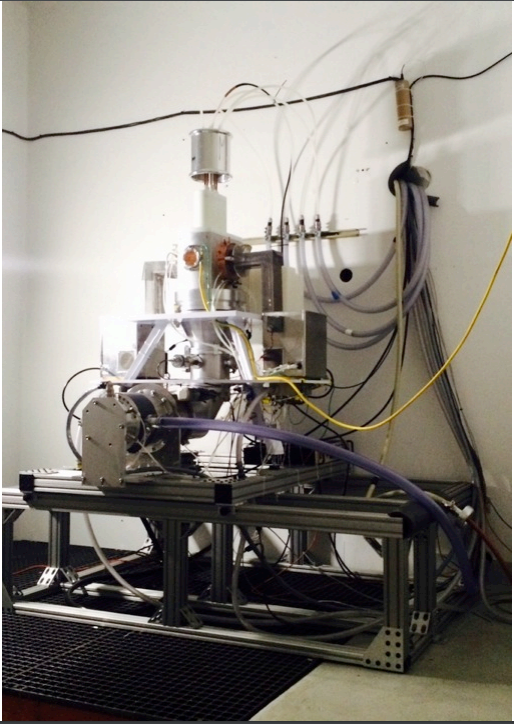
\includegraphics[width=\columnwidth]{./figures/Capture.PNG}
%         \subfigimg[width=0.496\textwidth]{}{./figures/57Co_cum.pdf}{50}
% %         \caption{ Decay curve for the $\beta^+$ decay of \ce{^{64}Cu}.}
% %         \refstepcounter{subfigure} 
% %         \label{fig:85gY}
%    \hspace{-10pt}}%
%     \\
%     \subfloat{
%         \centering
% %         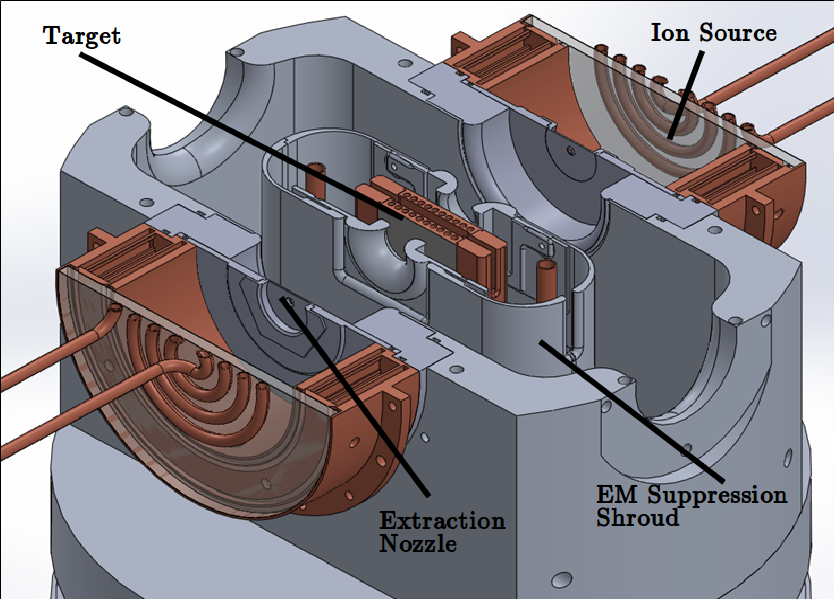
\includegraphics[width=\textwidth]{./figures/target2.png}
%         \subfigimg[width=0.496\textwidth]{}{./figures/60Co.pdf}{50}
% %         \caption{Decay curve for the $\beta^-$ decay of \ce{^{116}In}.}
%         %         \refstepcounter{subfigure}
% %          \label{fig:85mY}
% %    }
% %      \subfloat{
% %         \centering
% % %         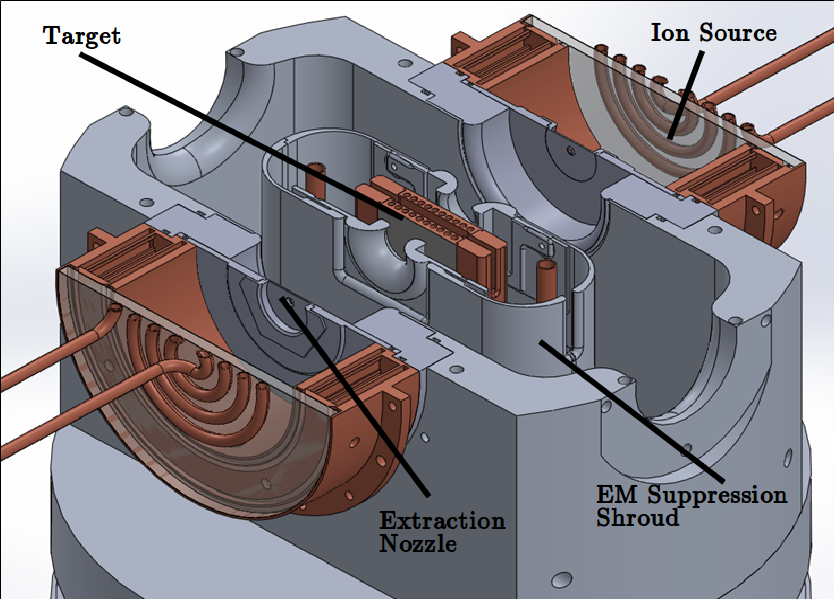
\includegraphics[width=\textwidth]{./figures/target2.png}
% %         \subfigimg[width=0.496\textwidth]{}{./figures/86Y.pdf}{50}
% % %         \caption{Decay curve for the $\beta^-$ decay of \ce{^{116}In}.}
% %         %         \refstepcounter{subfigure}
% %          \label{fig:86Y}
% %    }
% %     \\
% %     \subfloat{
% %         \centering
% %         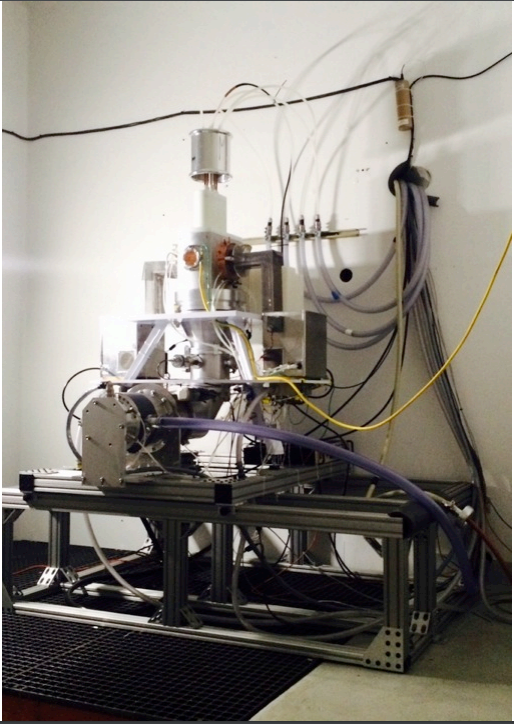
\includegraphics[width=\columnwidth]{./figures/Capture.PNG}
%         \subfigimg[width=0.496\textwidth]{}{./figures/60Cu.pdf}{50}
% %         \caption{ Decay curve for the $\beta^+$ decay of \ce{^{64}Cu}.}
% %         \refstepcounter{subfigure}
% %         \label{fig:86Zr}
%    \hspace{-10pt}}%
%     \\
%     \subfloat{
%         \centering
% %         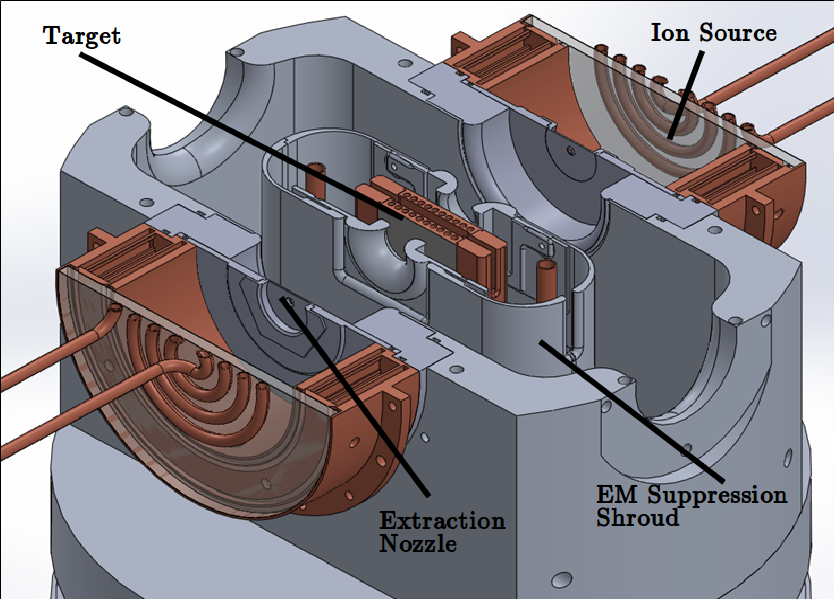
\includegraphics[width=\textwidth]{./figures/target2.png}
%         \subfigimg[width=0.496\textwidth]{}{./figures/61Co.pdf}{50}
% %         \caption{Decay curve for the $\beta^-$ decay of \ce{^{116}In}.}
%         %         \refstepcounter{subfigure}
% %          \label{fig:87Y}
% %    }
% %     \subfloat{
% %         \centering
% %         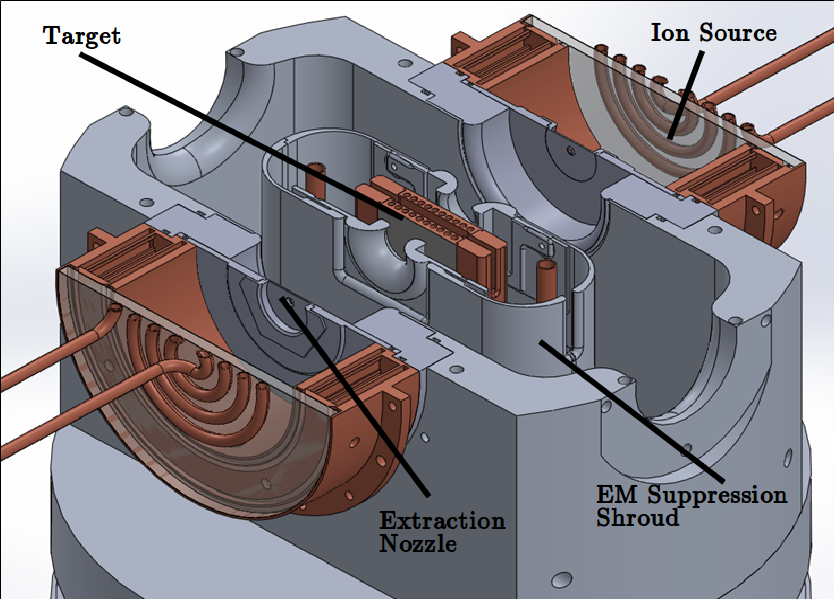
\includegraphics[width=\textwidth]{./figures/target2.png}
%         \subfigimg[width=0.496\textwidth]{}{./figures/61Cu.pdf}{50}
% %         \caption{Decay curve for the $\beta^-$ decay of \ce{^{116}In}.}
%         %         \refstepcounter{subfigure}
% %          \label{fig:87gY}
%    \hspace{-10pt}}
% %     \caption{Decay curves used to verify photopeak transition assignment. (a) Decay curve for the isomeric transition of \ce{^{115m}In}, (b) decay curve for the isomeric transition of \ce{^{113m}In}, (c) decay curve for the $\beta^-$ decay of \ce{^{116}In}, and (d) decay curve for the $\beta^+$ decay of \ce{^{64}Cu}.}
%      \phantomcaption{}\label{fig:xs_curves_p4}
% \end{figure*}
% 
% \begin{figure*}
%     \centering
%      \subfloat{
%         \centering
% % %         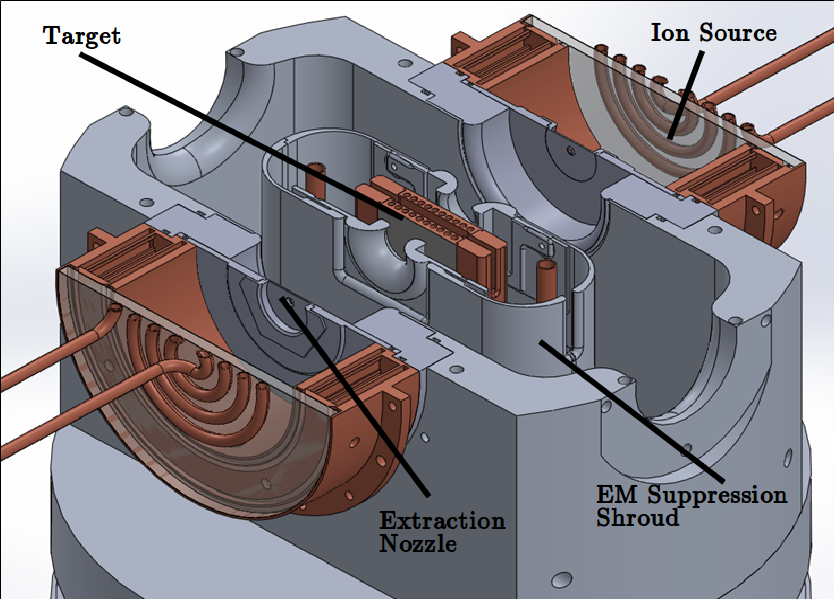
\includegraphics[width=\textwidth]{./figures/target2.png}
% %         \subfigimg[width=0.496\textwidth]{}{./figures/87gY.pdf}{50}
% % %         \caption{Decay curve for the $\beta^-$ decay of \ce{^{116}In}.}
% %         %         \refstepcounter{subfigure}
% %          \label{fig:87gY}
% % %    }
% %     \subfloat{
% %         \centering
% %         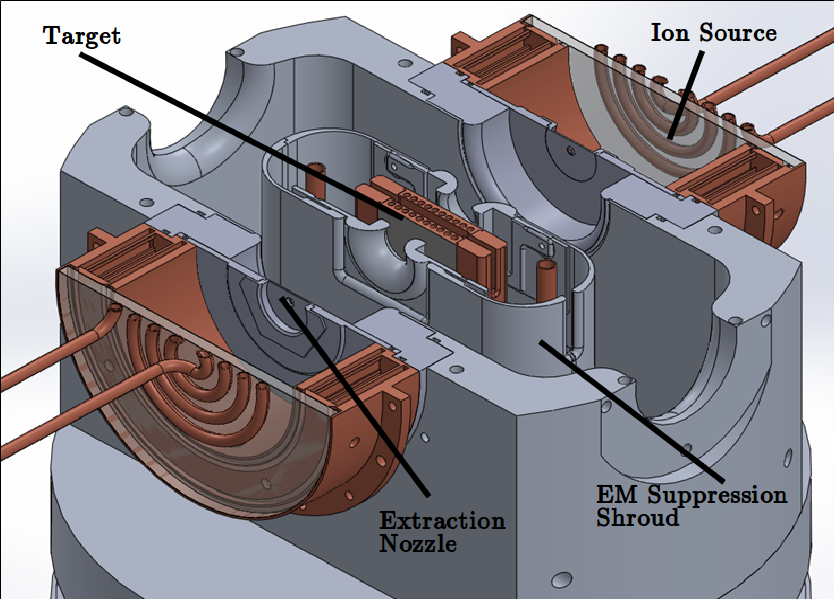
\includegraphics[width=\textwidth]{./figures/target2.png}
%         \subfigimg[width=0.496\textwidth]{}{./figures/64Cu.pdf}{50}
% %         \caption{Decay curve for the $\beta^-$ decay of \ce{^{116}In}.}
%         %         \refstepcounter{subfigure}
% %          \label{fig:87mY}
% %    }
% %     \subfloat{
% %         \centering
% %         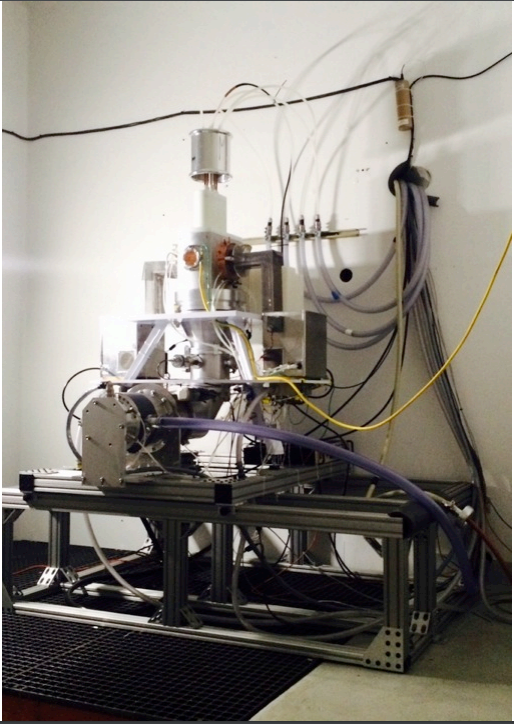
\includegraphics[width=\columnwidth]{./figures/Capture.PNG}
%         \subfigimg[width=0.496\textwidth]{}{./figures/43K.pdf}{50}
% %         \caption{ Decay curve for the $\beta^+$ decay of \ce{^{64}Cu}.}
% %         \refstepcounter{subfigure}
% %         \label{fig:87Zr}
%    \hspace{-10pt}}%
%     \\
%     \subfloat{
%         \centering
% %         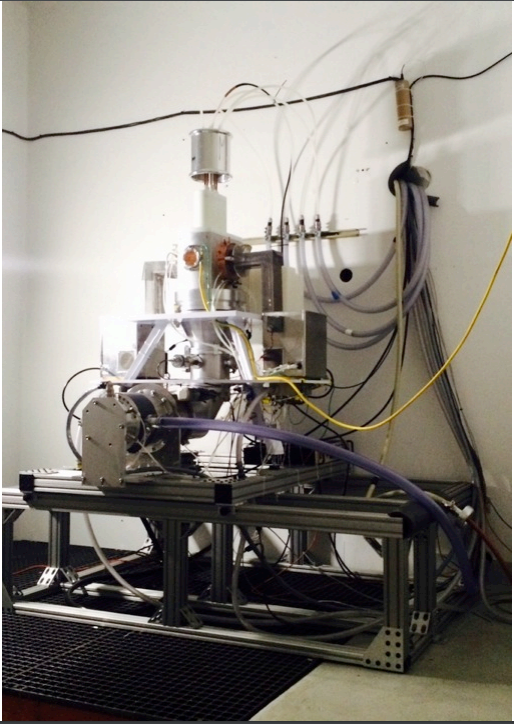
\includegraphics[width=\columnwidth]{./figures/Capture.PNG}
%         \subfigimg[width=0.496\textwidth]{}{./figures/44mSc.pdf}{50}
% %         \caption{ Decay curve for the isomeric transition of \ce{^{115m}In}.}
% %         \refstepcounter{subfigure}
% %          \label{fig:88Y}%
% %         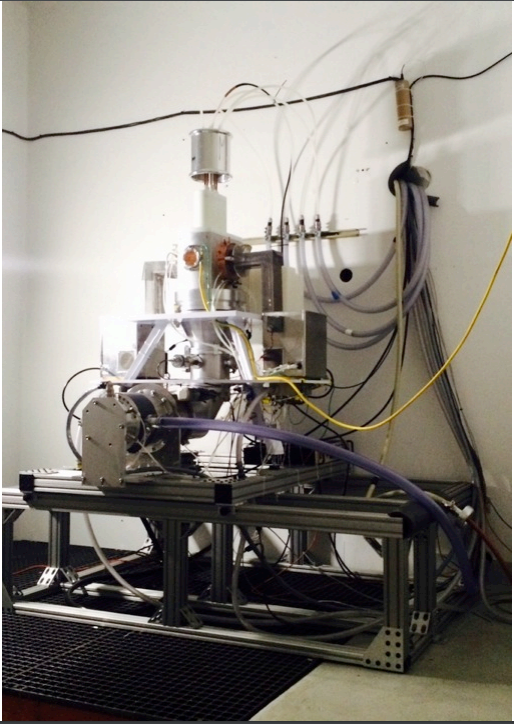
\includegraphics[width=\columnwidth]{./figures/Capture.PNG}
% %         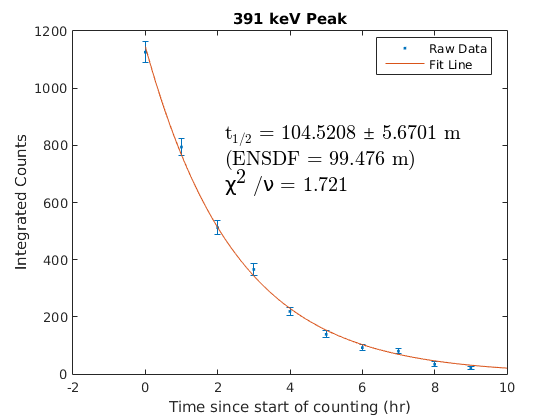
\includegraphics[scale=0.6]{./figures/391keV_curve2.png}
%         \subfigimg[width=0.496\textwidth]{}{./figures/44gSc.pdf}{50}
% %         \caption{ Decay curve for the isomeric transition of \ce{^{113m}In}.}
% %         \refstepcounter{subfigure}
% %          \label{fig:88Zr}
%    \hspace{-10pt}}%
%     \\
%          \subfloat{
%         \centering
% %         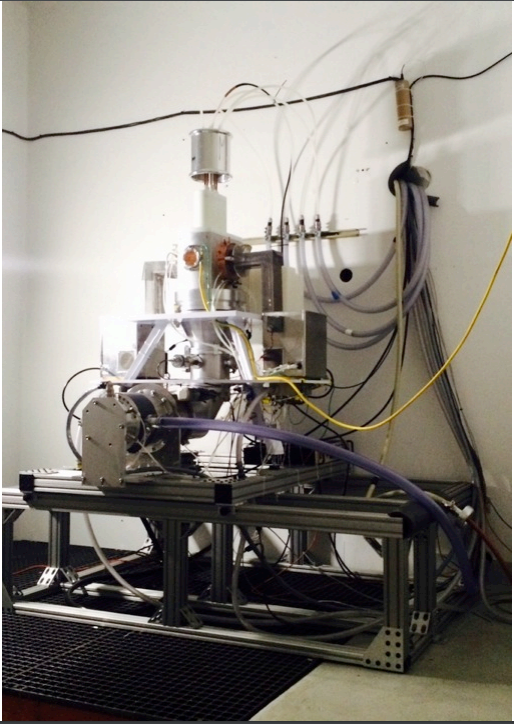
\includegraphics[width=\columnwidth]{./figures/Capture.PNG}
% %         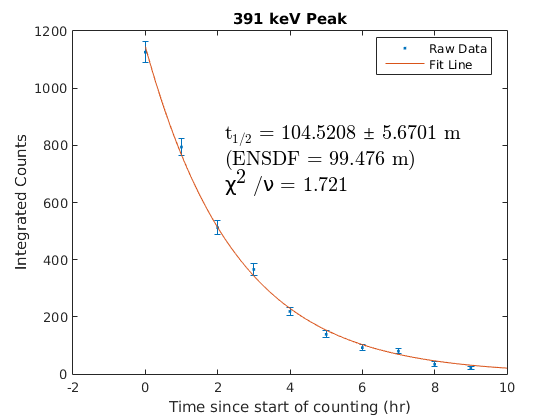
\includegraphics[scale=0.6]{./figures/391keV_curve2.png}
%         \subfigimg[width=0.496\textwidth]{}{./figures/44Sc.pdf}{50}
% %         \caption{ Decay curve for the isomeric transition of \ce{^{113m}In}.}
% %         \refstepcounter{subfigure}
% %          \label{fig:89Nb}
% %    }%
% %     \subfloat{
% %         \centering
% %         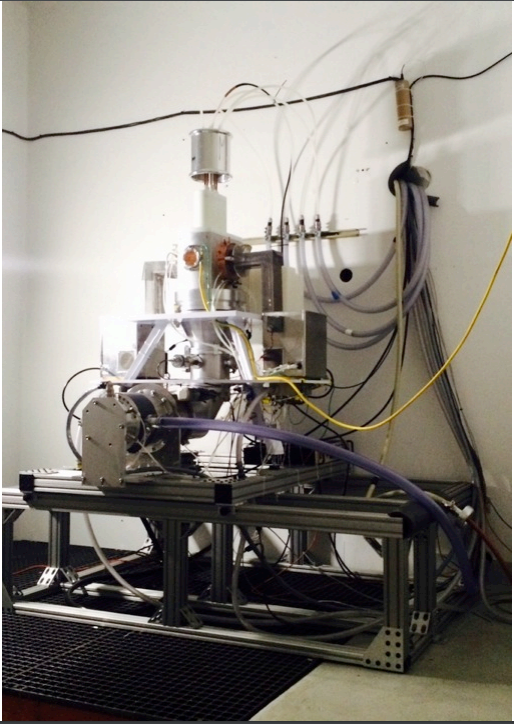
\includegraphics[width=\columnwidth]{./figures/Capture.PNG}
% %         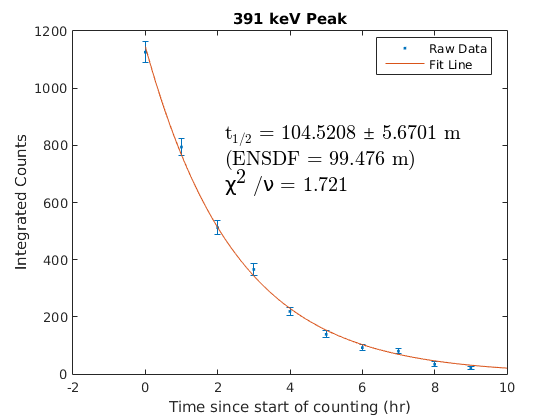
\includegraphics[scale=0.6]{./figures/391keV_curve2.png}
%         \subfigimg[width=0.496\textwidth]{}{./figures/47Sc.pdf}{50}
% %         \caption{ Decay curve for the isomeric transition of \ce{^{113m}In}.}
% %         \refstepcounter{subfigure}
% %          \label{fig:89gNb}
%    \hspace{-10pt}}%
% %     \caption{Decay curves used to verify photopeak transition assignment. (a) Decay curve for the isomeric transition of \ce{^{115m}In}, (b) decay curve for the isomeric transition of \ce{^{113m}In}, (c) decay curve for the $\beta^-$ decay of \ce{^{116}In}, and (d) decay curve for the $\beta^+$ decay of \ce{^{64}Cu}.}
%      \phantomcaption{}\label{fig:xs_curves_p8}
% % \caption{}
% \end{figure*}
% % 
% \begin{figure*}
%     \centering    
%          \subfloat{
%         \centering
% % %         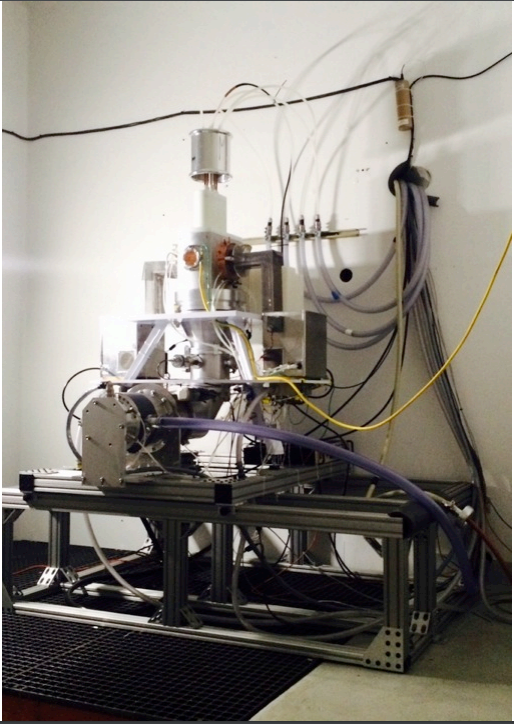
\includegraphics[width=\columnwidth]{./figures/Capture.PNG}
% % %         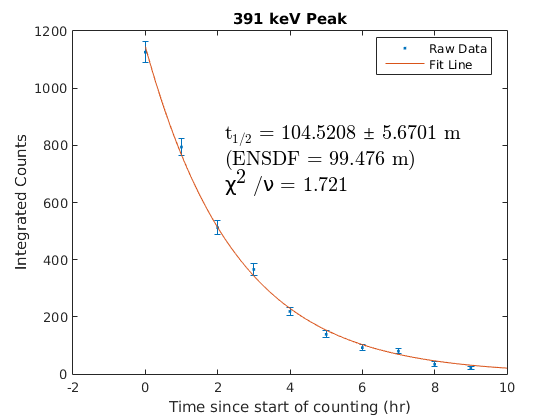
\includegraphics[scale=0.6]{./figures/391keV_curve2.png}
% %         \subfigimg[width=0.497\textwidth]{}{./figures/89gNb.pdf}{50}
% % %         \caption{ Decay curve for the isomeric transition of \ce{^{113m}In}.}
% % %         \refstepcounter{subfigure}
% %          \label{fig:89gNb}
% % %    }%
% %     \subfloat{
% %         \centering
% %         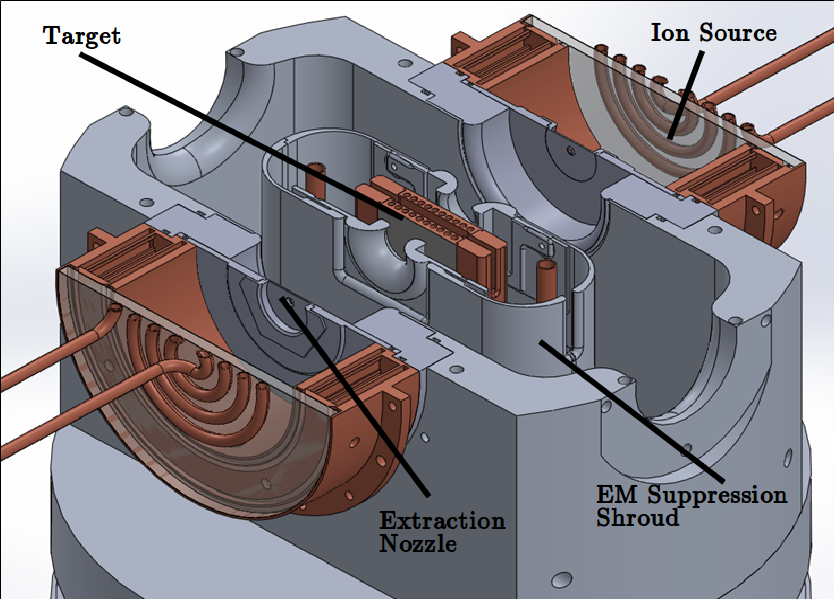
\includegraphics[width=\textwidth]{./figures/target2.png}
%         \subfigimg[width=0.497\textwidth]{}{./figures/48Sc.pdf}{50}
% %         \caption{Decay curve for the $\beta^-$ decay of \ce{^{116}In}.}
%         %         \refstepcounter{subfigure}
% %          \label{fig:89mNb}
% % %    }
% % %      \subfloat{
% % %         \centering
% % %         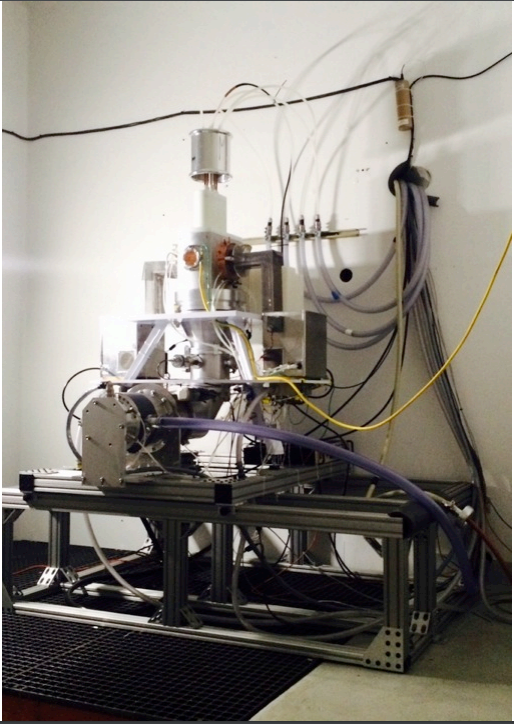
\includegraphics[width=\columnwidth]{./figures/Capture.PNG}
% %         \subfigimg[width=0.497\textwidth]{}{./figures/89Zr.pdf}{50}
% % %         \caption{ Decay curve for the $\beta^+$ decay of \ce{^{64}Cu}.}
% % %         \refstepcounter{subfigure} 
% % %         \label{fig:89Zr}
% %    \hspace{-10pt}}%
% %     \\
% %     \subfloat{
% %         \centering
% % %         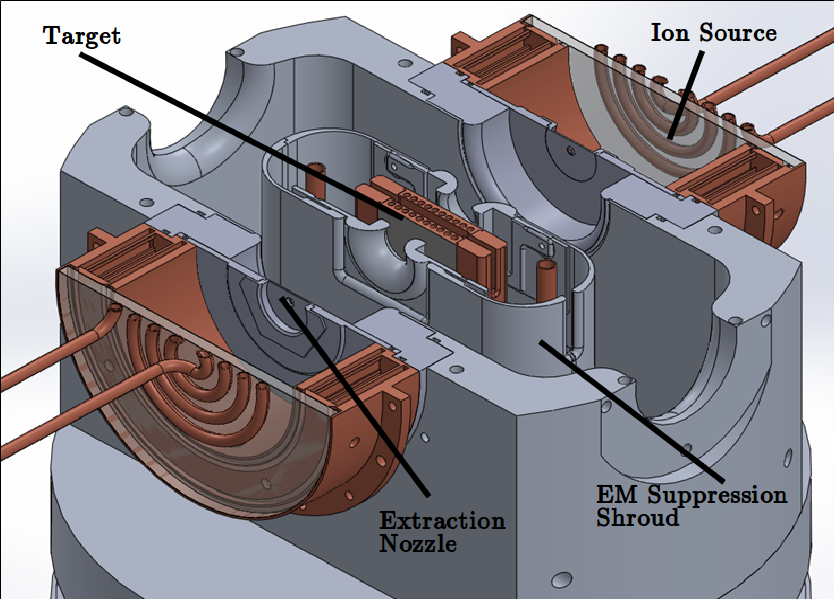
\includegraphics[width=\textwidth]{./figures/target2.png}
% %         \subfigimg[width=0.497\textwidth]{}{./figures/91mNb.pdf}{50}
% % %         \caption{Decay curve for the $\beta^-$ decay of \ce{^{116}In}.}
% %         %         \refstepcounter{subfigure}
% % %          \label{fig:91mNb}
% % %    }
% % %      \subfloat{
% % %         \centering
% % %         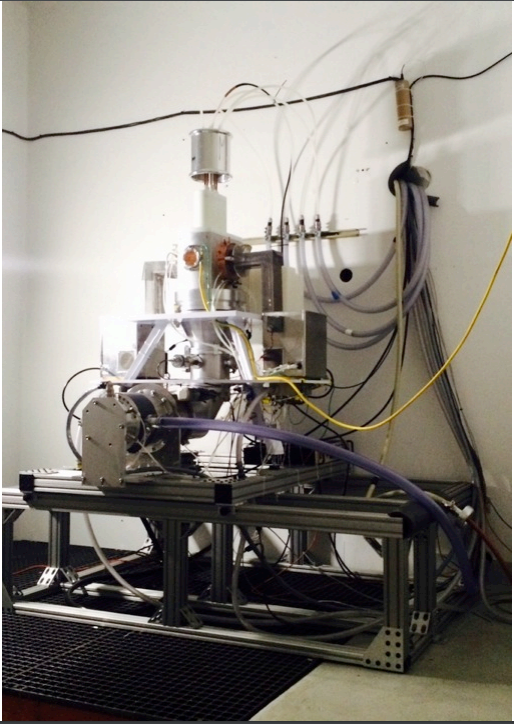
\includegraphics[width=\columnwidth]{./figures/Capture.PNG}
% %         \subfigimg[width=0.497\textwidth]{}{./figures/92mNb.pdf}{50}
% % %         \caption{ Decay curve for the $\beta^+$ decay of \ce{^{64}Cu}.}
% % %         \refstepcounter{subfigure} 
% % %         \label{fig:92mNb}
% %    \hspace{-10pt}}%
% %     \\
% %     \subfloat{
% %         \centering
% % %         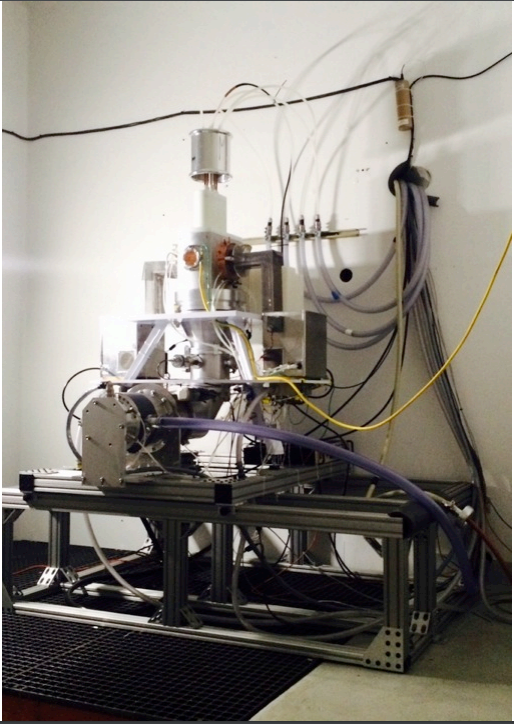
\includegraphics[width=\columnwidth]{./figures/Capture.PNG}
% %         \subfigimg[width=0.497\textwidth]{}{./figures/93mMo.pdf}{50}
% % %         \caption{ Decay curve for the isomeric transition of \ce{^{115m}In}.}
% % %         \refstepcounter{subfigure}
% % %          \label{fig:93mMo}
%    }%
% %     \caption{Decay curves used to verify photopeak transition assignment. (a) Decay curve for the isomeric transition of \ce{^{115m}In}, (b) decay curve for the isomeric transition of \ce{^{113m}In}, (c) decay curve for the $\beta^-$ decay of \ce{^{116}In}, and (d) decay curve for the $\beta^+$ decay of \ce{^{64}Cu}.}
%      \phantomcaption{}\label{fig:xs_curves_p7}
% % \caption{}
% \end{figure*}
% % 
% % % \begin{figure*}
% % %     \centering
% % %     \subfloat{
% % %         \centering
% % % %         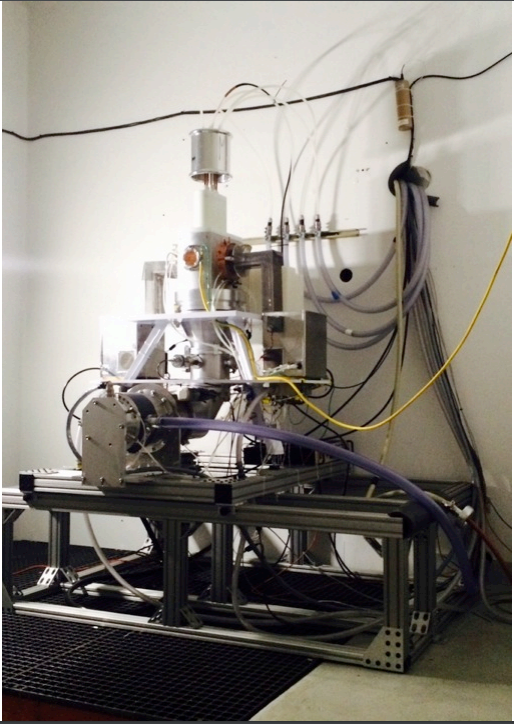
\includegraphics[width=\columnwidth]{./figures/Capture.PNG}
% % %         \subfigimg[width=0.497\textwidth]{}{./figures/93mMo.pdf}{50}
% % % %         \caption{ Decay curve for the isomeric transition of \ce{^{115m}In}.}
% % % %         \refstepcounter{subfigure}
% % %          \label{fig:93mMo}
% % %    }%
% % % %      \subfloat{
% % % %         \centering
% % % % %         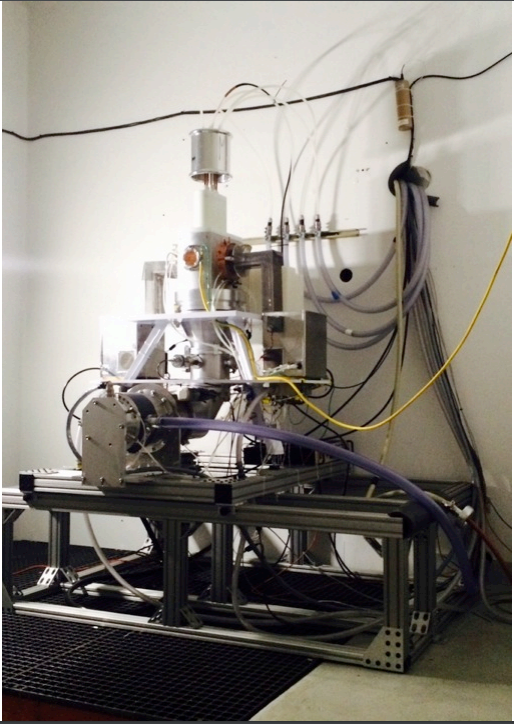
\includegraphics[width=\columnwidth]{./figures/Capture.PNG}
% % % % %         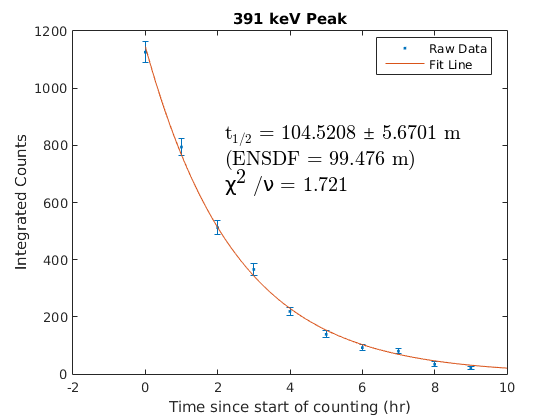
\includegraphics[scale=0.6]{./figures/391keV_curve2.png}
% % % %         \subfigimg[width=0.497\textwidth]{}{./figures/91mNb.pdf}{50}
% % % % %         \caption{ Decay curve for the isomeric transition of \ce{^{113m}In}.}
% % % % %         \refstepcounter{subfigure}
% % %          \label{fig:91mNb}
% % % %    }%
% % % %     \\
% % % %     \subfloat{
% % % %         \centering
% % % % %         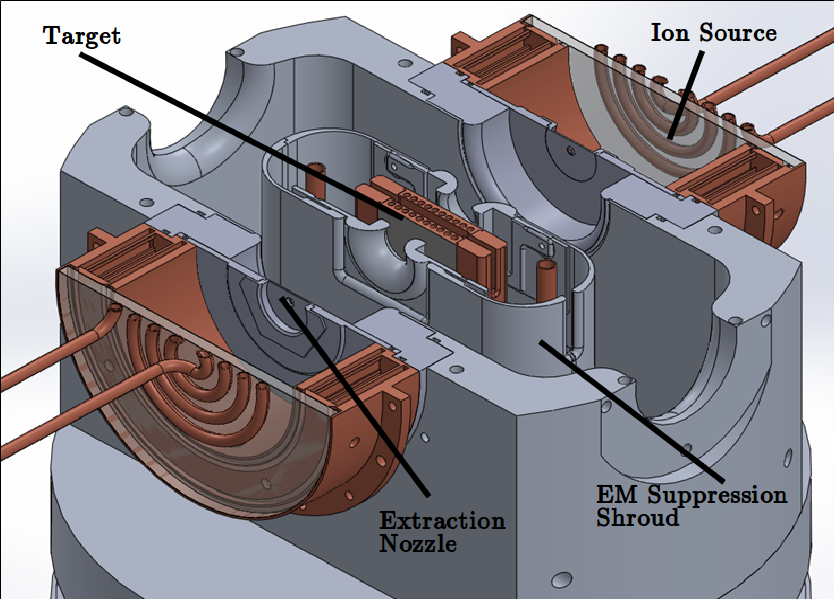
\includegraphics[width=\textwidth]{./figures/target2.png}
% % % %         \subfigimg[width=0.497\textwidth]{}{./figures/92mNb.pdf}{50}
% % % % %         \caption{Decay curve for the $\beta^-$ decay of \ce{^{116}In}.}
% % % %         %         \refstepcounter{subfigure}
% % %          \label{fig:92mNb}
% % % %    }
% % % %      \subfloat{
% % % %         \centering
% % % % %         \includegraphics[width=\columnwidth]{./figures/Capture.PNG}
% % % %         \subfigimg[width=0.497\textwidth]{}{./figures/93mMo.pdf}{50}
% % % % %         \caption{ Decay curve for the $\beta^+$ decay of \ce{^{64}Cu}.}
% % % %%         \refstepcounter{subfigure} \label{fig:93mMo}
% % % %    }%
% % % %     \caption{Decay curves used to verify photopeak transition assignment. (a) Decay curve for the isomeric transition of \ce{^{115m}In}, (b) decay curve for the isomeric transition of \ce{^{113m}In}, (c) decay curve for the $\beta^-$ decay of \ce{^{116}In}, and (d) decay curve for the $\beta^+$ decay of \ce{^{64}Cu}.}
% % %      \label{fig:xs_curves_p5}
% % % \end{figure*}
% % 
% % 


\pagebreak

\vspace{-20cm}


% 
% 
\section{Measured isomer-to-ground state branching ratios } \label{sec:U5_d_ibr_figures}

Plots of the isomer-to-ground state ratios measured in this work are presented here, in comparison with literature data and reaction modeling codes 
\cite{Michel1978,Kopecky1993,Zarie2006a,Khandaker2009}.



% 
%      
% 
% \begin{figure*}
%     \centering
%     \subfloat{
%         \centering
% % %         \includegraphics[width=\columnwidth]{./figures/Capture.PNG}
%         \subfigimg[width=0.497\textwidth]{}{./figures/52Mn_IBR.pdf}{50}
% % %         \caption{ Decay curve for the isomeric transition of \ce{^{115m}In}.}
% %         \refstepcounter{subfigure}
% %          \label{fig:52Mn_IBR}%
% %         \includegraphics[width=\columnwidth]{./figures/Capture.PNG}
% %         \includegraphics[scale=0.6]{./figures/391keV_curve2.png}
%         \subfigimg[width=0.497\textwidth]{}{./figures/58Co_IBR.pdf}{50}
% %         \caption{ Decay curve for the isomeric transition of \ce{^{113m}In}.}
% %         \refstepcounter{subfigure}
% %          \label{fig:58Co_IBR}
%    \hspace{-10pt}}%
%     \\
%     \subfloat{
%         \centering
% %         \includegraphics[width=\textwidth]{./figures/target2.png}
%         \subfigimg[width=0.497\textwidth]{}{./figures/44Sc_IBR.pdf}{50}
% %         \caption{Decay curve for the $\beta^-$ decay of \ce{^{116}In}.}
%         %         \refstepcounter{subfigure}
% %          \label{fig:85Y_IBR}
% %    }
% % %      \subfloat{
% % %         \centering
% % %         \includegraphics[width=\columnwidth]{./figures/Capture.PNG}
% %         \subfigimg[width=0.497\textwidth]{}{./figures/87Y_IBR.pdf}{50}
% % %         \caption{ Decay curve for the $\beta^+$ decay of \ce{^{64}Cu}.}
% % %         \refstepcounter{subfigure} 
% % %         \label{fig:87Y_IBR}
% %    \hspace{-10pt}}%
% %     \\
% %     \subfloat{
% %         \centering
% % %         \includegraphics[width=\textwidth]{./figures/target2.png}
% %         \subfigimg[width=0.497\textwidth]{}{./figures/89Nb_IBR.pdf}{50}
% % %         \caption{Decay curve for the $\beta^-$ decay of \ce{^{116}In}.}
% %         %         \refstepcounter{subfigure}
% % %          \label{fig:89Nb_IBR}
%    }
%      \phantomcaption{}\label{fig:ibr_curves}
% % \caption{}
% \end{figure*}


% \pagebreak

% 
% % 
% % 
% \section{Stack design } \label{sec:fe_stack_design}
% 
% % Plots of the isomer-to-ground state ratios measured in this work are presented here, in comparison with literature data and reaction modeling codes 
% % \cite{Michel1978,Kopecky1993,Zarie2006a,Khandaker2009}.
% 
% 
% 
% 
% 
% % Combined table
% % Please add the following required packages to your document preamble:
% % \usepackage{booktabs}
% \begin{table*}[h!]
% \centering
% \caption{Specifications of the 25\,MeV and 55\,MeV target stack designs in the present work. The proton beam enters the stack upstream of the SS-5 and SS-3 profile monitors, respectively, and travels through the stack in the order presented here. The 6061 aluminum degraders have a measured density of approximately 2.68 $\pm$ 0.03 g/cm$^3$. Their areal densities were determined using the variance minimization techniques described  in this work  and an earlier paper\,\cite{Voyles2018a}. 
% % the earlier paper by Graves \etal\\,\cite{Graves2016}.
% A 316 stainless steel foil is inserted at both the front and rear of each target stack as a monitor of the beam's spatial profile, by developing radiochromic film (Gafchromic EBT3) after end-of-bombardment (EoB).}
% \label{tab:fe_stack_table}
% \small
% \resizebox{\textwidth}{!}{%
% \begin{tabular}{@{}llll|llll@{}}
% \toprule\toprule
% % Target Layer       & Nominal Thickness & Measured thickness (mg/cm\textasciicircum 2) & Thickness Uncertainty (\%) \\ \midrule
% 25\,MeV Target layer            & \begin{tabular}[c]{@{}l@{}}Measured \\ thickness\end{tabular} & \begin{tabular}[c]{@{}l@{}}Measured\\areal density\\(mg/cm$^2$)\end{tabular} & \begin{tabular}[c]{@{}l@{}}Uncertainty \\ in areal\\ density  (\%)\end{tabular} & 55\,MeV Target layer            & \begin{tabular}[c]{@{}l@{}}Measured \\ thickness\end{tabular} & \begin{tabular}[c]{@{}l@{}}Measured\\areal density\\(mg/cm$^2$)\end{tabular} & \begin{tabular}[c]{@{}l@{}}Uncertainty \\ in areal\\ density  (\%)\end{tabular} \\
% \midrule
% SS profile monitor SS-5 & 130.94 \mmicro m                                              & 100.57                                                                      & 0.17                                                                      & SS profile monitor SS-3 & 130.9 \mmicro m                                               & 100.48                                                                      & 0.17                                                                      \\
% Fe-08                   & 26.25 \mmicro m                                               & 19.69                                                                       & 0.17                                                                      & Fe-01                   & 25.75 \mmicro m                                               & 20.22                                                                       & 0.21                                                                      \\
% Ti-14                   & 25.01 \mmicro m                                               & 10.87                                                                       & 0.36                                                                      & Ti-01                   & 25.88 \mmicro m                                               & 11.09                                                                       & 0.16                                                                      \\
% Cu-14                   & 24.01 \mmicro m                                               & 17.49                                                                       & 0.40                                                                      & Cu-01                   & 28.81 \mmicro m                                               & 22.40                                                                       & 0.11                                                                      \\
% Al Degrader E-09        & 256.5 \mmicro m                                               & --                                                                          & --                                                                        & Al Degrader A-1         & 2.24 mm                                                       & --                                                                          & --                                                                        \\
% Fe-09                   & 26.5 \mmicro m                                                & 19.90                                                                       & 0.09                                                                      & Fe-02                   & 25.5 \mmicro m                                                & 19.91                                                                       & 0.13                                                                      \\
% Ti-15                   & 23.81 \mmicro m                                               & 10.97                                                                       & 0.11                                                                      & Ti-02                   & 25.74 \mmicro m                                               & 10.94                                                                       & 0.24                                                                      \\
% Cu-15                   & 21.81 \mmicro m                                               & 17.63                                                                       & 0.46                                                                      & Cu-02                   & 28.75 \mmicro m                                               & 22.32                                                                       & 0.40                                                                      \\
% Al Degrader H-01        & 127.09 \mmicro m                                              & --                                                                          & --                                                                        & Al Degrader A-2         & 2.24 mm                                                       & --                                                                          & --                                                                        \\
% Fe-10                   & 26.5 \mmicro m                                                & 19.84                                                                       & 0.11                                                                      & Fe-03                   & 25.25 \mmicro m                                               & 20.00                                                                       & 0.27                                                                      \\
% Ti-16                   & 24.6 \mmicro m                                                & 10.96                                                                       & 0.32                                                                      & Ti-03                   & 25.91 \mmicro m                                               & 11.25                                                                       & 0.15                                                                      \\
% Cu-16                   & 22.01 \mmicro m                                               & 17.22                                                                       & 0.25                                                                      & Cu-03                   & 28.86 \mmicro m                                               & 22.49                                                                       & 0.20                                                                      \\
% Fe-11                   & 27.26 \mmicro m                                               & 19.96                                                                       & 0.17                                                                      & Al Degrader C-1         & 0.97 mm                                                       & --                                                                          & --                                                                        \\
% Ti-17                   & 25.01 \mmicro m                                               & 10.88                                                                       & 0.25                                                                      & Fe-04                   & 25.25 \mmicro m                                               & 19.93                                                                       & 0.33                                                                      \\
% Cu-17                   & 29 \mmicro m                                                  & 21.91                                                                       & 0.33                                                                      & Ti-04                   & 25.84 \mmicro m                                               & 10.91                                                                       & 0.18                                                                      \\
% Fe-12                   & 27.01 \mmicro m                                               & 20.03                                                                       & 0.12                                                                      & Cu-04                   & 28.78 \mmicro m                                               & 22.38                                                                       & 0.29                                                                      \\
% Ti-18                   & 25.01 \mmicro m                                               & 11.00                                                                       & 0.87                                                                      & Al Degrader C-2         & 0.97 mm                                                       & --                                                                          & --                                                                        \\
% Cu-18                   & 28.75 \mmicro m                                               & 22.33                                                                       & 0.14                                                                      & Fe-05                   & 25.64 \mmicro m                                               & 20.02                                                                       & 0.24                                                                      \\
% Fe-13                  & 26.25 \mmicro m                                               & 20.05                                                                       & 0.16                                                                      & Ti-05                   & 25.86 \mmicro m                                               & 10.99                                                                       & 0.30                                                                      \\
% Ti-19                   & 26.6 \mmicro m                                                & 11.01                                                                       & 0.22                                                                      & Cu-05                   & 28.77 \mmicro m                                               & 22.35                                                                       & 0.12                                                                      \\
% Cu-19                   & 28.75 \mmicro m                                               & 22.32                                                                       & 0.19                                                                      & Al Degrader C-3         & 0.97 mm                                                       & --                                                                          & --                                                                        \\
% Fe-14                   & 25.75 \mmicro m                                               & 20.11                                                                       & 0.19                                                                      & Fe-06                   & 25.75 \mmicro m                                               & 20.21                                                                       & 0.26                                                                      \\
% Ti-20                   & 27.01 \mmicro m                                               & 11.06                                                                       & 0.35                                                                      & Ti-06                   & 25.5 \mmicro m                                                & 11.15                                                                       & 0.23                                                                      \\
% Cu-20                   & 28.26 \mmicro m                                               & 22.34                                                                       & 0.28                                                                      & Cu-06                   & 28.83 \mmicro m                                               & 22.43                                                                       & 0.10                                                                      \\
% SS profile monitor SS-6 & 131.5 \mmicro m                                               & 100.99                                                                      & 0.17                                                                      & Al Degrader C-4         & 0.97 mm                                                       & --                                                                          & --                                                                        \\
%                         &                                                               &                                                                             &                                                                           & Fe-07                   & 25.76 \mmicro m                                               & 19.93                                                                       & 0.19                                                                      \\
%                         &                                                               &                                                                             &                                                                           & Ti-07                   & 25.75 \mmicro m                                               & 11.17                                                                       & 0.33                                                                      \\
%                         &                                                               &                                                                             &                                                                           & Cu-07                   & 28.76 \mmicro m                                               & 22.34                                                                       & 0.24                                                                      \\
%                         &                                                               &                                                                             &                                                                           & Al Degrader H-02        & 127.04 \mmicro m                                              & --\cmmnt{34.51}                                                                       & --\cmmnt{0.20}                                                                      \\
%                         &                                                               &                                                                             &                                                                           & SS profile monitor SS-4 & 131.21 \mmicro m                                              & 101.25                                                                      & 0.16                                                                     \\
%  \bottomrule\bottomrule
% \end{tabular}
% }
% \end{table*}


\pagebreak
